\section{Ensemble Network}
 Ensembling consists of pooling together the predictions of a set of different models to produce better predictions. Nowadays, in every machine learning competitions, in particular on Kaggle, the winners use very large ensembles of models that inevitably beat any single model, no matter how good, hence we decided to use it also in our project.
 
 
Ensembling relies on the assumption that different well-performing models trained independently are likely to be good for different reasons: each model looks at slightly different aspects of the data to make its predictions, getting part of the “truth” but not all of it\footnote{This can be see in detail in the "data visualization" chapter}. By pooling the perspective of different models together, a far more accurate description of the data can be obtained.

\subsection{Our approach}
In our project we decided to use a simple ensembling approach, which is \textit{average voting}: average voting computes the average of the scores (i.e., softmax output) of the base classifiers and select the class with the highest score.

Although we decided to use this simple approach, even if it is very common, we decided to optimize the choice of models to be used in order to maximize the accuracy obtained on the testset. In fact, all the models described in the chapter "pre-trained models" have been saved as \textit{".keras"} models so that they can be reloaded and used to directly evaluate the testset in the ensemble, so that they do not need to be trained again (thus increasing the speed of test execution).

The main problem was to choose which of these models combined together obtained the best accuracy. Since the number of models was more than 20 a grid search seemed too slow as a method of solving this problem, so we decided to use a genetic algorithm to solve the problem automatically.




\subsubsection{The Ensemble Class}
To perform the ensemble in an orderly fashion, what was done was to create a class called \textit{Ensemble}. The class allows to construct, predict and evaluate in a simple way ensemble networks composed of different models. Here the code:

\begin{python}
class Ensemble:

    def __init__(self, test_images_vgg, test_images_resnet, test_images_inception):
        self.test_images_vgg = test_images_vgg
        self.test_images_resnet = test_images_resnet
        self.test_images_inception = test_images_inception

        # obtain original labels
        self.labels = np.array([])
        for x, y in self.test_images_vgg:
            self.labels = np.concatenate([self.labels, np.argmax(y.numpy(), axis=-1)])

        # create list of models
        self.model_list = []

        base_dir = './models/'
        # VGG16
        for name in vgg16:
            self.model_list.append(ks.models.load_model(base_dir + 'vgg16/' + name))

        # ResNet50
        for name in resnet50:
            self.model_list.append(ks.models.load_model(base_dir + 'resnet50/' + name))

        # ResNet50
        for name in resnet101:
            self.model_list.append(ks.models.load_model(base_dir + 'resnet101/' + name))

        # Inception
        for name in inception:
            self.model_list.append(ks.models.load_model(base_dir + 'inception/' + name))

        # compute all prediction once for all
        self.predictions = []
        for i, model in enumerate(self.model_list):
            if i < len(vgg16):
                self.predictions.append(model.predict(self.test_images_vgg))
            elif i < len(vgg16) + len(resnet50) + len(resnet101):
                self.predictions.append(model.predict(self.test_images_resnet))
            else:
                self.predictions.append(model.predict(self.test_images_inception))

    def predict(self, active_models):
        sum_prediction = None
        start = 0
        count = 0

        if np.sum(active_models) == 0:
            return None

        for start, active_model in enumerate(active_models):
            if active_model == 1:
                sum_prediction = self.predictions[start]
                count += 1
                break

        # additional model selected and added
        for i in range(start + 1, len(self.model_list)):
            if active_models[i] == 0:
                continue
            sum_prediction += self.predictions[i]
            count += 1

        print(count)
        final_preds = 1 / count * sum_prediction
        return np.argmax(final_preds, axis=1)

    def evaluate(self, predictions):
        if predictions == 0:
            return 0

        count = 0
        for i, prediction in enumerate(predictions):
            if int(self.labels[i]) == prediction:
                count += 1
        return count/len(self.labels)

    def predict_and_evaluate(self, active_models):
        return self.evaluate(self.predict(active_models))

    def labels_len(self):
        return len(self.labels)
\end{python}

The \textit{constructor} takes in input 3 datasets that are equal to each other except for the size of the images, in fact VGG, ResNet and Inception want in input images with size (256,256), (224, 244) and (299,299) respectively: this is done in order to correctly evaluate the models without having errors due to the input data. The constructor also computes the labels of each test sample, loads the models and computes the predictions for each of them, this is done to speed up the execution of the genetic algorithm.

Moving on to discuss the \textit{predict} function, it takes as input an array of length equal to the total number of models consisting of zeros or ones. The array indicates the models to be used: in the same position where a one is present the corresponding model inside {model\_list} must be used.

As for the \textit{evaluate} function, it takes an array of predictions and returns the accuracy, calculated as the number of correct predictions over the total number of test samples.

\subsubsection{Genetic Algorithm Workflow}
Following the guidelines in Section 2.6, we need to decide how to develop the different components and decide on the hyperparameters in order to define the flow of the genetic algorithm.

\paragraph{Genotype}
In our specific case, our chromosomes are binary encoded and each gene represents a different model. Hence, we have individuals made of a number of genes equal to the number of different models that we have.

\begin{python}
# create an operator that randomly returns 0 or 1
toolbox.register('zeroOrOne', random.randint, 0, 1)

# define a single objective, maximizing fitness strategy:
creator.create('FitnessMax', base.Fitness, weights=(1.0,))

# create the Individual class based on list:
creator.create('Individual', list, fitness=creator.FitnessMax)

# create the individual operator to fill up an Individual instance:
toolbox.register('individualCreator', tools.initRepeat, creator.Individual, toolbox.zeroOrOne, INDIVIDUAL_LENGTH)
\end{python}

\paragraph{Population}
The population is composed of 100 individuals, we decided to keep a high number of individuals in order to have more chances to have more different individuals and therefore to have different starting points in order to converge better to the optimal solution. Although the number of individuals may seem very high, we decided to increase the speed of the computation of the prediction simply by calculating once and for all the values of the predictions for each classifier at the creation of the Ensemble class, and save them in memory for later use without having to recompute them.

\begin{python}
toolbox.register('populationCreator', tools.initRepeat, list, toolbox.individualCreator)
\end{python}

\paragraph{Fitness Function}
The fitness function is the accuracy obtained through the \textit{predict\_and\_evaluate} function of the Ensemble class. It was registered in the \textit{toolbox} as follows:

\begin{python}
def ensembleAccuracy(individual):
    return ensemble.predict_and_evaluate(individual)

toolbox.register('evaluate', ensembleAccuracy)
\end{python}

\paragraph{Selection Algorithm}
The selection algorithm used in this case is \textit{tournament selection}. In each round of the tournament selection method, two individuals are randomly picked from the population, and the one with the highest fitness score wins and gets selected. We decided to select only five individuals since our population is small and selecting more could cause an abuse in exploitation.

\begin{python}
# Tournament selection with tournament size of 5:
toolbox.register("select", tools.selTournament, tournsize=5)
\end{python}


\paragraph{Crossover Algorithm}
As crossover algorithm we decided to use the \textit{two-point crossover}. In the two-point crossover method, two crossover points on the chromosomes of both parents are selected randomly. The genes residing between these points are swapped between the two parent chromosomes.

The following diagram demonstrates a two-point crossover carried out on a pair of binary chromosomes, with the first crossover point located between the third and fourth genes, and the other between the seventh and eighth genes:

\begin{figure}[H]
	\centering
	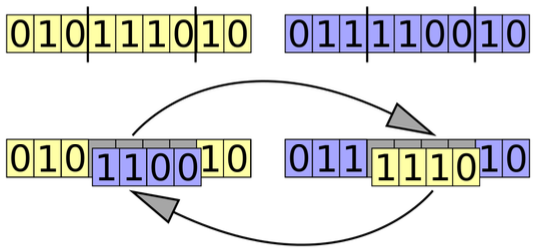
\includegraphics[width=0.4\textwidth]{img/twopointcross.png}
	\caption{Two point crossover example.}
	\label{fig:twopointcross}
\end{figure}

The code for that is:
\begin{python}
toolbox.register("mate", tools.cxTwoPoint)
\end{python}

\paragraph{Mutation Algorithm}
As mutation algorithm we decided to use the \textit{Multiple Flip bit mutation}. When applying the flip bit mutation to a binary chromosome, one gene is randomly selected and its value is flipped (complemented), as shown in the following diagram:

\begin{figure}[H]
	\centering
	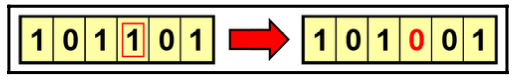
\includegraphics[width=0.4\textwidth]{img/flipbit.png}
	\caption{Flip bit mutation example.}
	\label{fig:flipbit}
\end{figure}

This can be extended to several random genes being flipped instead of just one, obtaining the multiple flip bit mutation that we use.
The code for that is:
\begin{python}
toolbox.register("mutate", tools.mutFlipBit, indpb=1.0/INDIVIDUAL_LENGTH)
\end{python}


\paragraph{Elitism}
We set the number of individuals for the elitism mechanism to 5. This value has been chosen in consideration of the fact that the number of individuals is 100, not very high, and that an individual is composed of little more than twenty genes: if we chose a higher value for the hall of fame, what could happen is that we could not exploit much the global search carried out by the exploration because we would end up with very similar chromosomes; therefore, in order not to risk bad results, we chose to use this conservative approach and limit the number to these few.

\paragraph{GA Flow}
The first thing to do is to define the initial population, this is easily done by the following line of code:

\begin{python}
population  = toolbox.populationCreator(n=POPULATION_SIZE)
\end{python}

After that, we created a statistical object. This object has served to have a report of the flow of the genetic algorithm, allowing us to save for each generation the maximum and average fitness values obtained, so that we can show them once the generations are over.

\begin{python}
stats = tools.Statistics(lambda ind: ind.fitness.values)
stats.register("max", np.max)
stats.register("avg", np.mean)
\end{python}

Then, the last object we need to create for the \textit{eaSimple} is the \textbf{HallOfFame}, which can be done through the following line of code:

\begin{python}
hof = tools.HallOfFame(HALL_OF_FAME_SIZE)
\end{python}

The main flow is done using the \textit{eaSimple} in the way as follow:

\begin{python}
population, logbook = algorithms.eaSimple(population,
								  toolbox,
								  cxpb=P_CROSSOVER,
								  mutpb=P_MUTATION,
								  ngen=MAX_GENERATIONS,
								  stats=stats,
								  halloffame=hof,
								  verbose=True)
\end{python}

Where the P\_CROSSOVER is equal to 0.9, P\_MUTATION 0.1.\footnote{Value suggested by the book ”Hands on Genetic Algorithms with Python” by Eyal Wirsansky, also the other values of probabilities are taken by the suggestions of the book}
